\begin{figure}[H]
    \centering
    \label{fig:back-prop-example}
    
    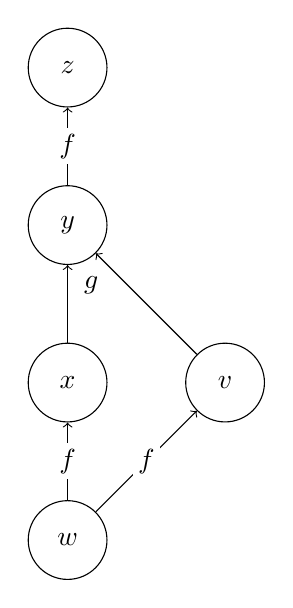
\begin{tikzpicture}
        \def\vert{2}
        \def\hori{2}
        \tikzstyle{place}=[circle, draw=black, minimum size=10mm]
        \tikzstyle{lbl}=[inner sep=2pt, fill=white]
        
        % Nodes
        \node[place] (w) at (0 * \hori, 0 * \vert) {\(w\)};

        \node[place] (x) at (0 * \hori, 1 * \vert) {\(x\)};
        \node[place] (v) at (1 * \hori, 1 * \vert) {\(v\)};
        
        \node[place, label={[shift={(0.3,-1.5)}]{\(g\)}}] (y) at (0 * \hori, 2 * \vert) {\(y\)};
        
        \node[place] (z) at (0 * \hori, 3 * \vert) {\(z\)};
        
        % Edges
        \draw [->] (w) to node[lbl]{\(f\)} (x);
        \draw [->] (w) to node[lbl]{\(f\)} (v);

        \draw [->] (x) to (y);
        \draw [->] (v) to (y);
        
        \draw [->] (y) to node[lbl]{\(f\)} (z);
        
    \end{tikzpicture}
    \caption{Example graph for back-propagation}
\end{figure}